\subsection{Подход математиков из Нижнего Новгорода}

В 2012 году математики А.А.Пономаренко, Ю.А.Мальков, А.А.Логвинов и В.В.Кры\-лов
опубликовали статью \cite{Ponomarenko} , в которой предложили свой подход к созданию графов со свойствами 
тесного мира. А также предоставили оптимизацию для алгоритма жадного поиска. Так как сама модель
очень сильно опирается на этот алгоритм, предлагаю начать изучение именно с него.

\subsubsection{Жадный поиск}
Данный алгоритм предназначен для эффективного поиска вершины в графе. Идейно он очень прост.
На каждой итерации цикла, мы смотрим все соседние вершины и идём к той, что ближе всего к цели.
Если таких вершин нет, то мы нашли то, что искали.

\begin{itemize}
    \item Преимуществом данного алгоритма является его быстродействие по сравнению с другими методами. 
    \item Недостаток же кроется в его неточности. Может существовать такая вершина от\-личная
    от нашей, соседи которой будут дальше от цели, чем она сама. Такие вер\-шины, как уже упоминалось,
    принято называть локальными минимумами 
\end{itemize}

Блок схему алгоритма можно увидеть на рис \ref{grady_search_block_scheme}. 

\begin{figure}[H]
    \centering
    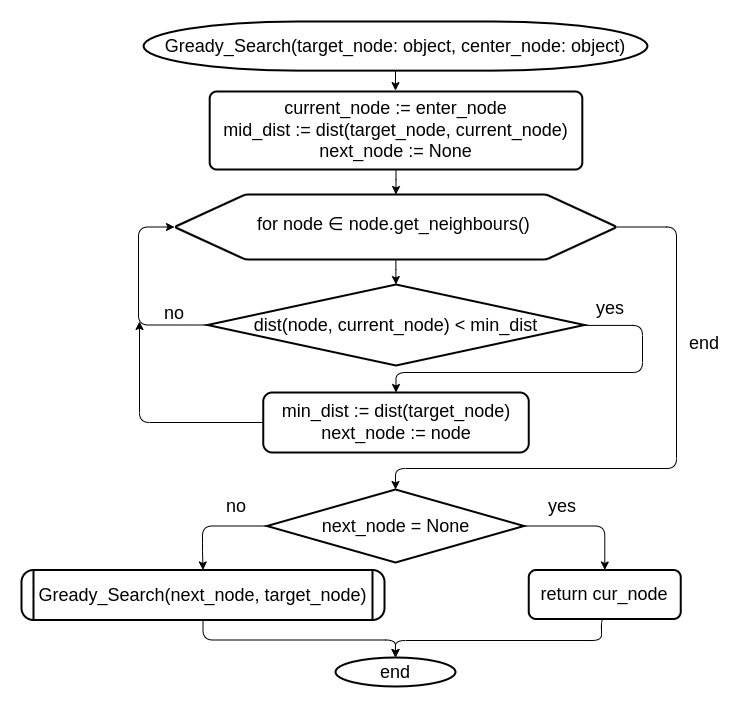
\includegraphics[scale=0.6]{./pictures/Gready_Search.png}
    \caption{Блок схема жадного поиска} \label{grady_search_block_scheme}
\end{figure}

Хочется подметить, что этот алгоритм относится к классу рандомизированных алго\-ритмов,
так как сам поиск мы начинаем в случайной вершине. На практике такой подход показывает
результат куда лучше, чем если бы стартовая вершина была детерминирован\-ной.


Математики из нижнего новгорода, упомянутые выше, предложили способ, как можно улучшить
данный алгоритм, уменьшив вероятность попадания в локальные минимумы. Его блок схему
вы можете найти на рис \ref{multi_search_block_scheme}. Идея заключается в том, чтобы
запустить жадный поиск несколько раз от произвольных вершин и выбрать ту, что окажется ближе.
Данный подход рационален, так как мы подразумеваем, что работаем в "Тесном" \ графе, а значит,
поиск не будет занимать много времени. Они также пришли к выводу, что достаточно делать
$m \approx \log{n}$ повторений

\begin{figure}[H]
    \centering
    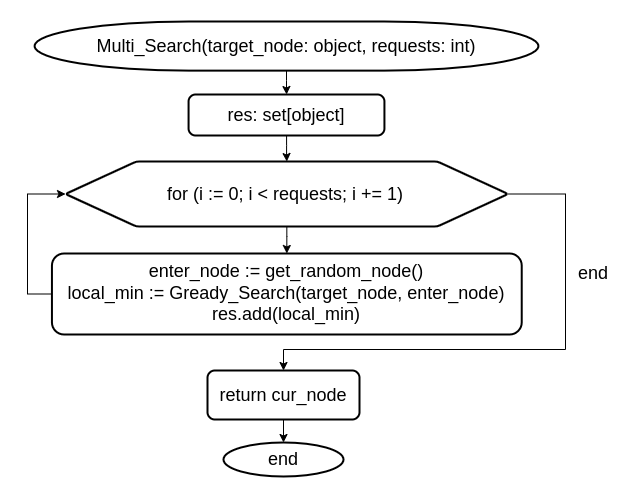
\includegraphics[scale=0.6]{./pictures/Multi_Search.png}
    \caption{Блок схема многократного жадного поиска} \label{multi_search_block_scheme}
\end{figure}

\subsubsection{Построение структуры}

Для построение структуры нам необходимо взять пустой граф и добавлять в него вершины
поэлементно, опираясь на следующий алгоритм: Перед добавлением новой вер\-шины v в граф, 
используя жадный поиск, мы ищем её потенциальное окружение (самые близкие к ней вершины,
присутствующие в графе на данный момент). Выбрав из них только k штук (здесь k - параметр, который
можно варьировать) связываем их с целевой вершиной v. Блок схему данного Алгоритма можно
увидеть на рис \ref{Ponomarenko_graph_block_scheme}.

\begin{figure}[H]
    \centering
    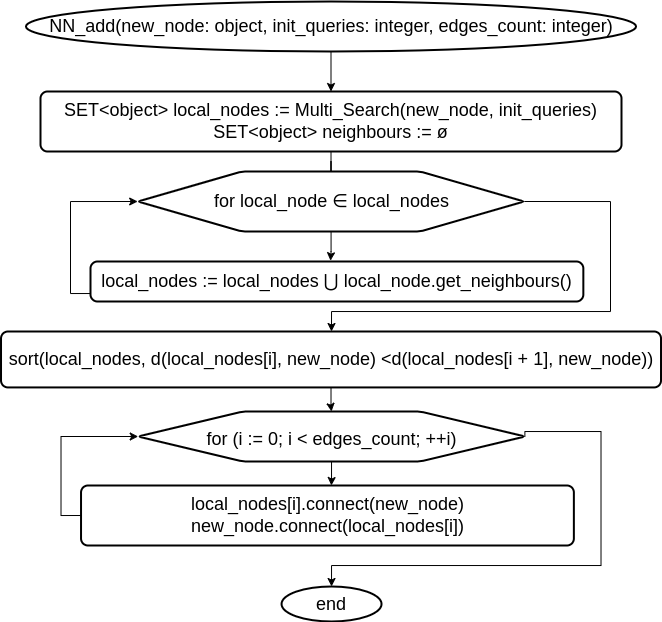
\includegraphics[scale=0.6]{./pictures/Ponomarenko_add_node.png}
    \caption{Блок схема построение структуры NNGraph} \label{Ponomarenko_graph_block_scheme}
\end{figure}

Хочется подметить несколько важных аспектов:
\begin{itemize}
    \item Граф сильно кластеризован по определению, так как мы связываем вершины только 
    с их ближайшими соседями
    \item Во время создания структуры, данные должны приходить случайно! Игнорирование 
    этого требования может привести к увеличению среднего диаметра
\end{itemize}

Поподробнее остановимся на втором пункте. \\ 
Рассмотрим граф, изображённый на рис \ref{lattice}:

\begin{figure}[H]
    \centering
    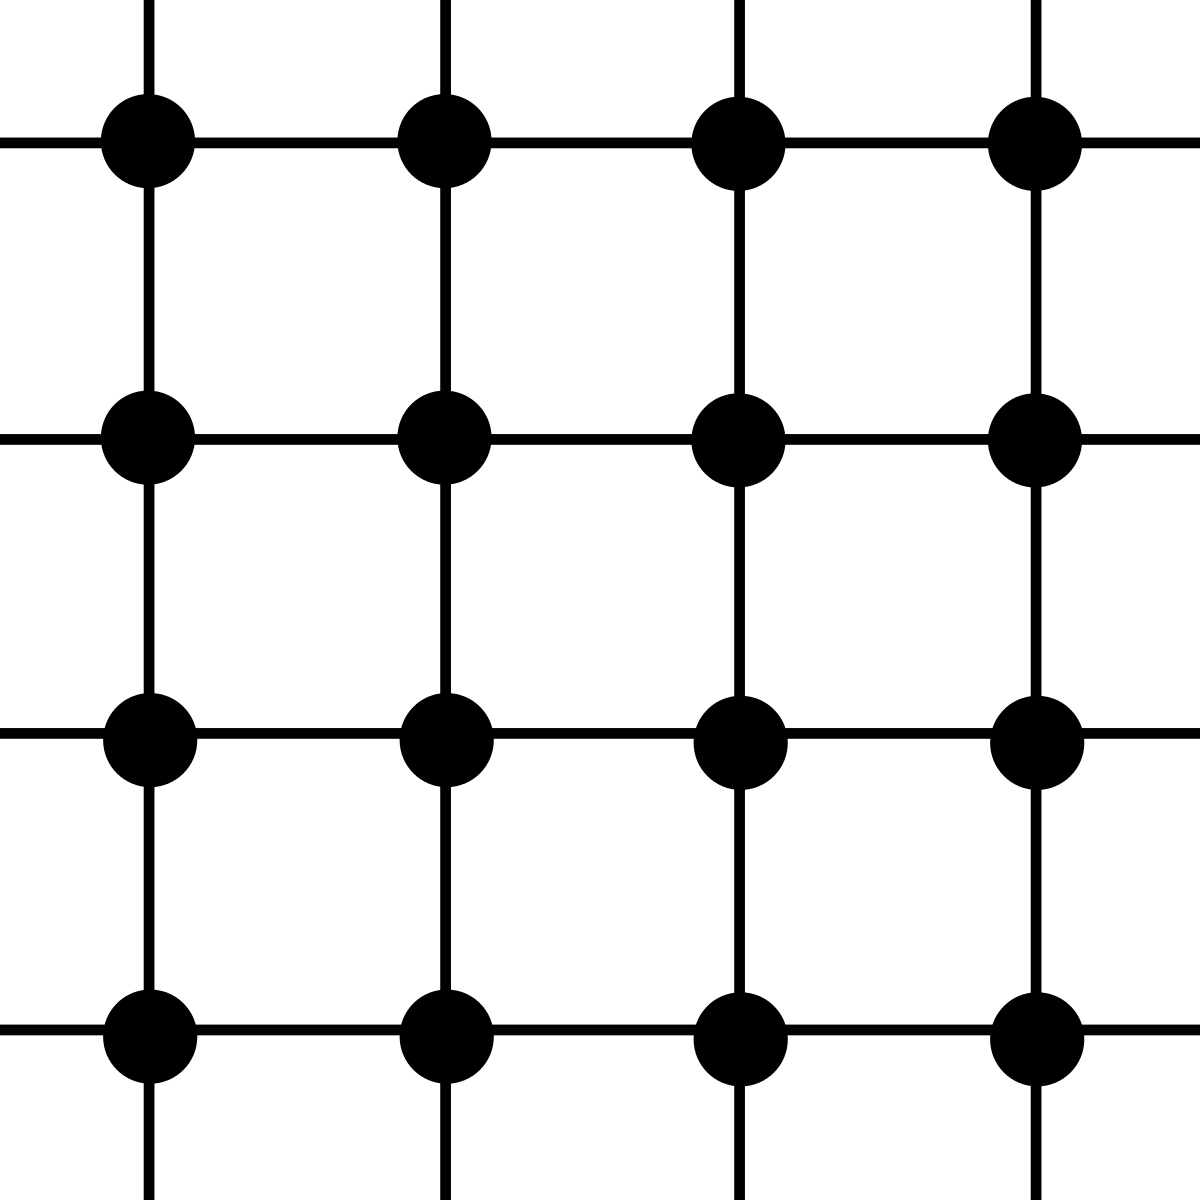
\includegraphics[scale=0.1]{./pictures/Square_grid_graph.svg.png}
    \caption{Пример } \label{lattice}
\end{figure}

Заметим, что даже такой крохотный пример уже имеет средний диаметр $= 2.375$.
Если мы увеличим сетку в 16 раз, то получим средний диаметр $= 9.5$. То есть мы пришли к тому,
что этот граф на 256 вершинах будет иметь средний диаметр больше, чем реальный
граф с 8 млрд вершинами. Но это ещё не всё, заметим, что коэфицент класстеризации тут 
вовсе равен нулю. Так что, этот пример не просто слабо похож на тесный граф, а является 
его полной противоположностью.

Для понимания, как случайность спасает нас в данной ситуации, разделим построение
графа на 2 части:
\begin{itemize}
    \item В самом начале формирование графа, вершин в нём будет немного. Случайный поток данных
    приведёт к тому, что узлы будут достаточно далеко друг от друга (вероятность
    обратного пренебрежимо мала). Поэтому Ближайшие соседи вершины v, которые будут найдены
    посредством жадного алгоритма, будут хоть и самыми близкими из текущих, однако всё
    ещё будут находиться на достаточно большом расстоянии к v. 
    \item С течением времени, ситуация начнёт меняться, ведь вершин будет становиться всё больше,
    а значит, и расположены они будут куда плотнее. Вершины добавленные под конец формирования графа,
    будут иметь соседей, которые будут к ним очень близки не только в сравнении с другими, но и
    по абсолютной величине.
\end{itemize}

Другими словами, в в самом начале формирования графа образуются длинные связи, которые помогают
быстро перемещаться по графу, а ближе к концу - короткие, которые спасают от локальных минимумов.